
\documentclass[12pt,a4paper]{report}
\usepackage[english]{babel}
\usepackage[T1]{fontenc}
\usepackage{times}
\usepackage{amsmath}
\usepackage{amsfonts}
\usepackage{amssymb}
\usepackage{textcomp}
\usepackage{gensymb}
\usepackage{hyperref}
\usepackage{graphicx}
\usepackage{setspace}
\usepackage[version=4]{mhchem}
\usepackage{caption}
\usepackage{subcaption}
\usepackage{longtable}
\usepackage[dvipsnames]{xcolor}
\usepackage{tikz}
\usepackage{wrapfig}
\usepackage[left=2cm,right=2cm,top=2cm,bottom=2cm]{geometry}
\makeatletter
\newcommand\footnoteref[1]{\protected@xdef\@thefnmark{\ref{#1}}\@footnotemark}
\makeatother
\graphicspath{{IMAGE/}}

    \makeatletter
\newcommand{\AlignFootnote}[1]{%
  \ifmeasuring@
  \else
    \iffirstchoice@
      \footnote{#1}%
    \fi
  \fi}
\makeatother



\begin{document}

\begin{titlepage}

\centering

\includegraphics[scale=0.25]{logo_ulg.png}%

\begin{center}\bfseries\huge
\vspace*{1cm}
Modeling and design of electromagnetic systems
\end{center}

\begin{center}\normalsize
Professor: C. Geuzaine\\
\end{center}

\vspace*{\stretch{1}}
\hrulefill
\begin{center}\bfseries\Huge
Homework 3 
\end{center}

\hrulefill
\vspace*{1cm}
\begin{center}\bfseries\Large
Sour Nassim, Heylen Martin
\end{center}

\begin{center}\bfseries\large

Master in electromechanical engineering\\ Bloc 2 \\
University of Liège \\
Academic year: 2019-2020
\end{center}
\vspace*{\stretch{2}}
\begin{flushright}

\end{flushright} 

\end{titlepage}
\setstretch{1.5}
\chapter{Introduction}
\quad\, This project is dedicated to the study of three-phase transformers. Those components are essential in the electrical network to switch from one voltage value to an other, or to reroute some part of the power to equaly distribute the power flow through the different branches of the network. Figure \ref{fig:real_transformer} shows the picture of a typical three-phase transformer.

\begin{figure}[h]
    \centering
    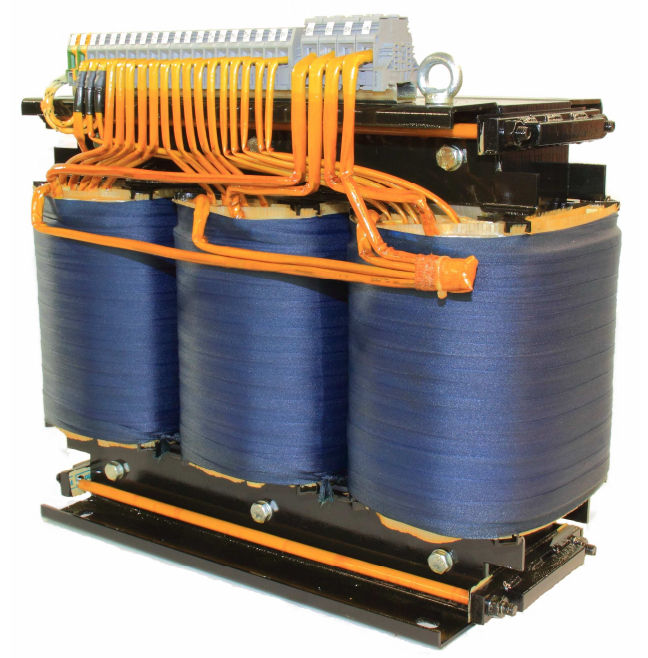
\includegraphics[width=0.4\textwidth]{real_transfo.jpg}
    \caption{Example of real three-phase transformer}
    \label{fig:real_transformer}
\end{figure}
\newpage
\chapter{Upstream analysis}
In this chapter will be introduced all the required elements to conduct the analysis of the studied three-phase transformers. Here, two transformers, respectively named \textbf{A} and \textbf{B}), of two different sizes will be considered in this report. The first one is a small transformer that makes the voltage going from 2.4 kV to 240 V for a nominal apparent power of 200 kVA. Let's define the transformer ratio $N$ as being the ratio between the secondary and the primary terminal voltage values. For this transformer, the transformer ratio is equal to 

\begin{equation}
\setstretch{1}
    N_A = \frac{240}{2400}\cdot 100 = 10\%
\end{equation}

The second transformer is bigger since it works between the 60 kV and 2.4 kV (leading to a transformer ratio of 4\%). The nominal apparent power of this transformer is equal to 20,000 KV.

These characteristics supposed that the network is at 50 Hz. Those are summarized in Table \ref{tab:characteristics_transfo}.

\begin{table}[h]
    \centering
\begin{tabular}{l|ll}
Transformer type   & \textbf{A}             & \textbf{B} \\ \hline
Input voltage [V]  & 2400                   & 60000      \\
Output voltage [V] & 240                    & 2400       \\
Output power [kVA] & 200                    & 20000      \\
Frequency [Hz]     & \multicolumn{1}{c}{50} & 50        
\end{tabular}
    \caption{Specifications of the two three-phase transformers}
    \label{tab:characteristics_transfo}
\end{table}

In the statement of the project, there is no information about if the given voltages are phase-to-phase or phase-to-neutral. Also, it is not indicated if those are peak or RMS values. Therefore, it will be assumed that the specified voltage are phase-to-phase RMS voltage.

Therefore, the nominal apparent power $S_N$ is defined as follows

\begin{equation}
\setstretch{1}
    S_N = \sqrt{3}\cdot U_N\cdot I_N
\end{equation}

where $U_N$ is the nominal phase-to-phase voltage (RMS value) and $I_N$ is the nominal current (RMS value).
\section{Type of three-phase transformer}
\quad\, When considering a three phase transformer, several configurations regarding to the construction of the core.

The first type of transformer consists in connecting three single-phase transformers together. This configuration is suitable for transformers of large nominal power. Also, "in case of failure of one of the transformers, only that transformer is replaced"\footnote{\url{http://www.montefiore.ulg.ac.be/~vct/elec0014/transp-t.pdf}}. It is also easier to carry.

The second type of three-phase transformers are ones for which the core is shared for the three phases. Thus, this implies that the phases are coupled together.

Also, the "volume of this common core is smaller than three times the volume of a single core".

In this project, the magnetic material used for the core is soft iron for which the saturation induction is around 2T. Also, since it has been said that three individuals core were more suitable for big transformers, transformer \textbf{B} will be design in this way.

\section{Choice of the three-phase transformer connections}
\quad\, Once the core(s) is(are) designed, the second step is to make a decision regarding to the type of connection of the different phases. Basically, considering one side of the transformer, the winding can either be connected in \textcolor{red}{star} or \textcolor{green}{delta}.
\subsection{Star connection}
\quad\, The star connection consists in connecting each of three phases to a common nodes which is usually grounded. The star connection is depicted on Figure \ref{fig:star}.
\begin{figure}[h]
    \centering
    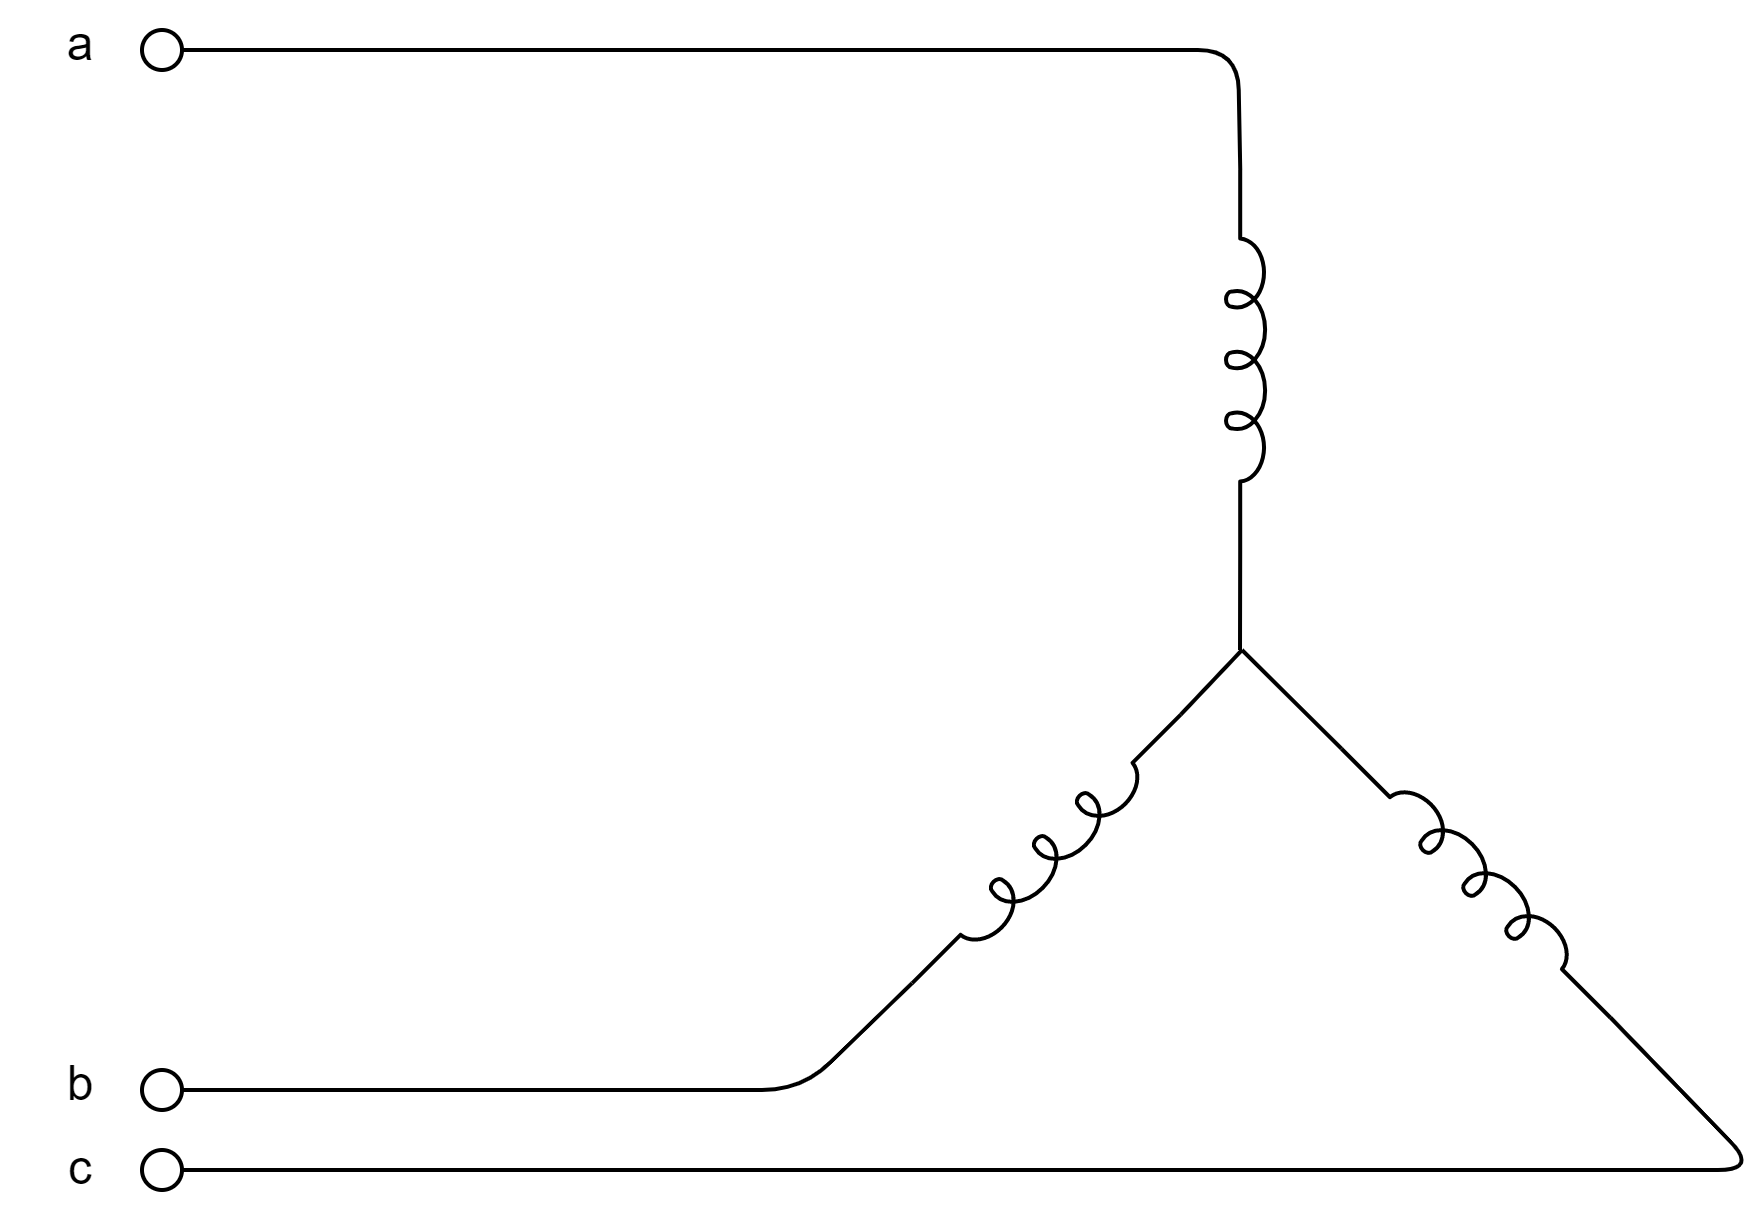
\includegraphics[width=0.5\textwidth]{Star.png}
    \caption{Three phase device - Star connection}
    \label{fig:star}
\end{figure}

The advantages of this type of connection are multiple. First, in case of a fault, the really high current generated due to this fault can be evacuated through this grounding connecting. Also, the star connection are usually used for the high voltage side of the transformer because it allows to cut by $\sqrt{3}$ the voltage in each phase of the transformer.

\subsection{Delta connection}
The second type of connection of the three phases are delta connection. Here, the each extremities of a winding are connected to the two others phases, creating a closed loop. The delta configuration is illustrated on Figure \ref{fig:delta}.

\begin{figure}[h]
    \centering
    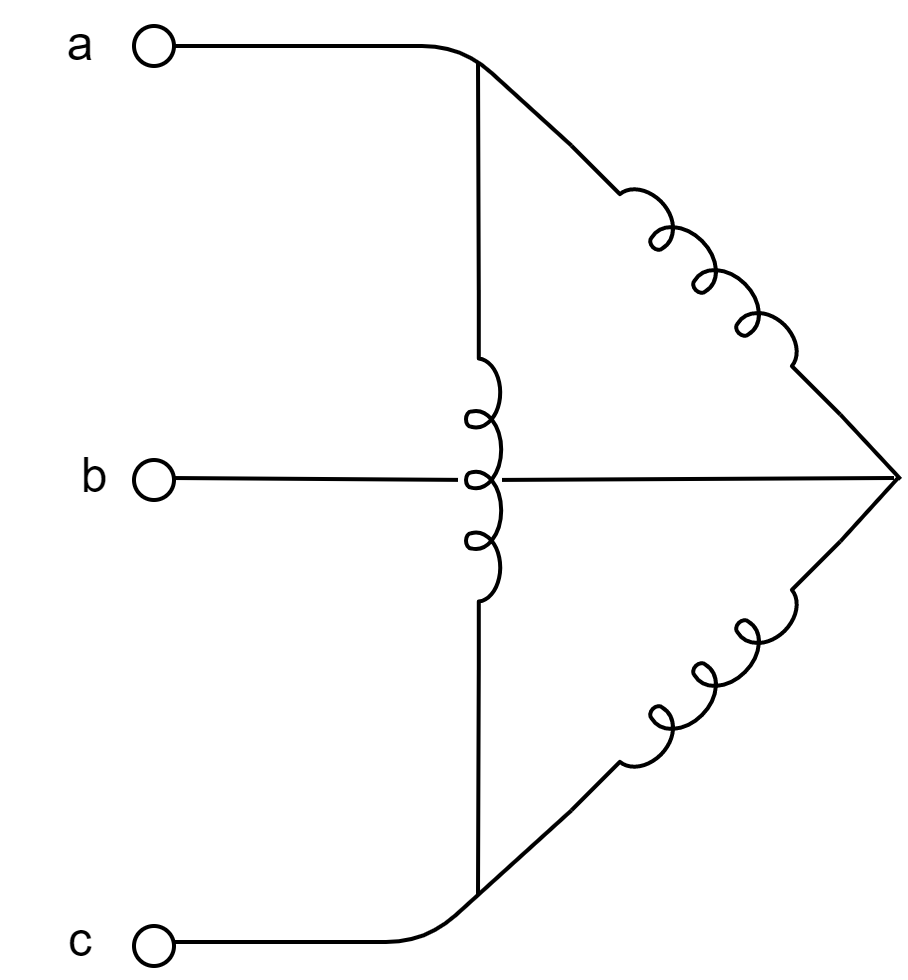
\includegraphics[width=0.5\textwidth]{Delta.png}
    \caption{Three phase device - Star connection}
    \label{fig:delta}
\end{figure}

Considering a current of intensity I injected in each lines \textit{a}, \textit{b}, and \textit{c}, it can be demonstrated that the current flowing through the branches of the transformer is $\sqrt{3}$ smaller.

Usually, when considering a three-phase transformer, the connections at the low voltage side follow the delta type to minimize the current flowing in the winding of the transformer.
\newpage
\subsection{Transformer - Possible mountings}
\quad\, The two previous subsections described the two possible type of connection of a three-phase device. Considering a transformer, the primary and secondary sides can be both considered as two three-phase devices. Thus, there are four possible mountings for the transformer.

\begin{itemize}
    \item Star-Star: The primary and secondary sides are both connected in star. This configuration, that can be met for high-voltage (HV) phase-shifting transformer, is depicted in Figure \ref{fig:star-star transformer}. 
    \begin{figure}[h]
    \centering
    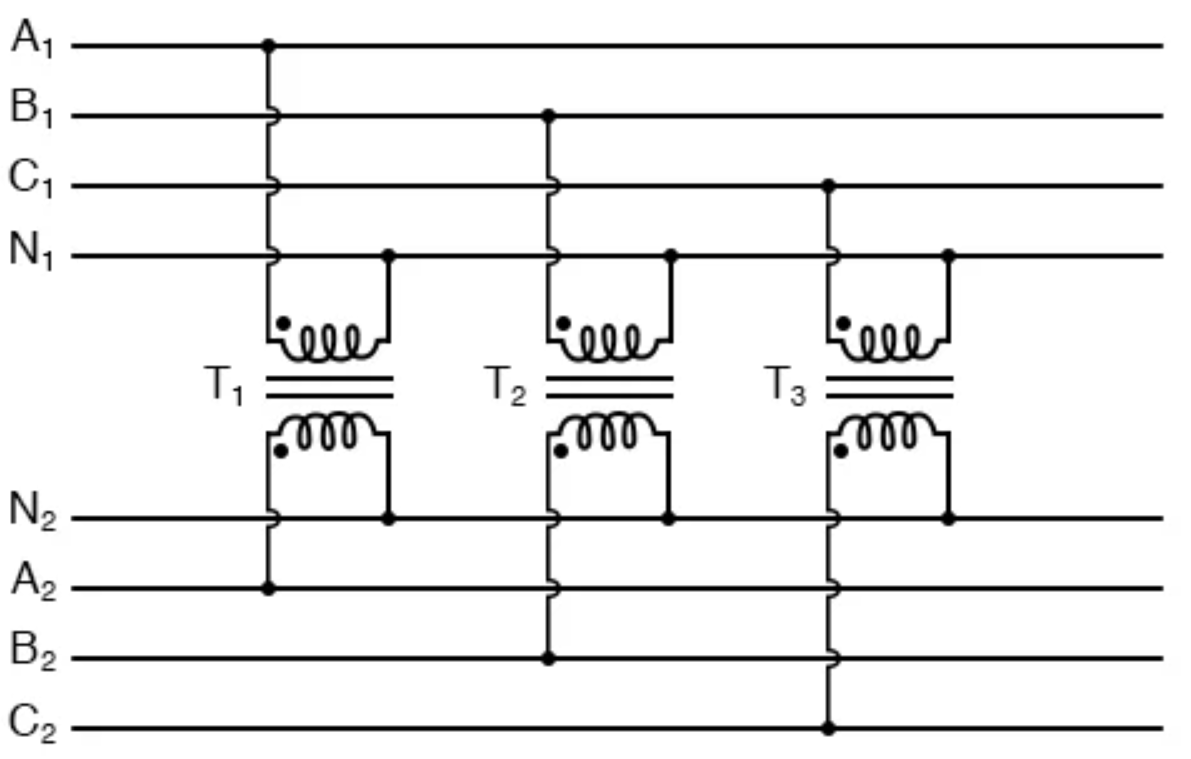
\includegraphics[width=0.6\textwidth]{y-y.PNG}
    \caption{Star-Star three-phase transformer}
    \label{fig:star-star transformer}
    \end{figure}
    
    \item Delta-Delta: The primary and secondary sides are both connected in delta. This configuration, that can be met for low-voltage (LV) phase-shifting transformer, is depicted in Figure \ref{fig:delta-delta transformer}. 
    \begin{figure}[h]
    \centering
    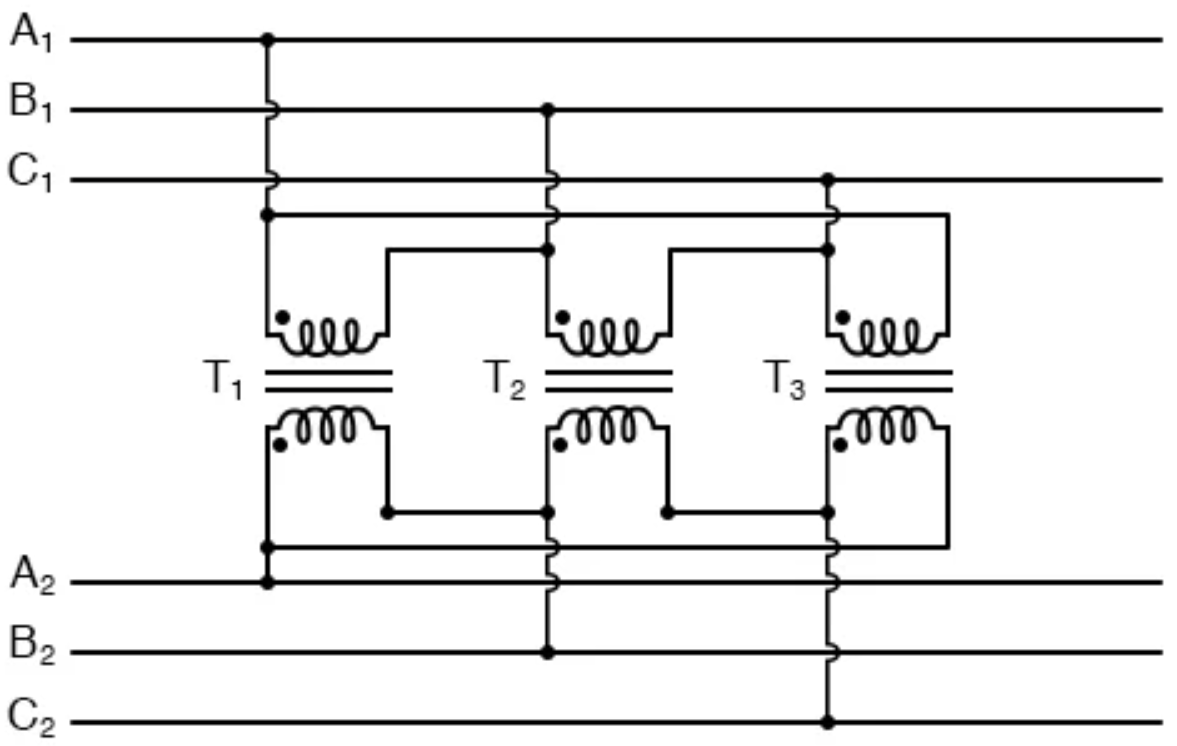
\includegraphics[width=0.6\textwidth]{delta-delta.PNG}
    \caption{Delta-Delta three-phase transformer}
    \label{fig:delta-delta transformer}
    \end{figure}
\end{itemize}
\newpage
\begin{itemize}
    \item Delta-Star: The primary side is wired in delta while the secondary side follows the star configuration. Delta-Star transformers are often used for step-up transformer because high current will flows in the primary side. Figure \ref{fig:delta-star transformer} depicts such configuration. 
    \begin{figure}[h]
    \centering
    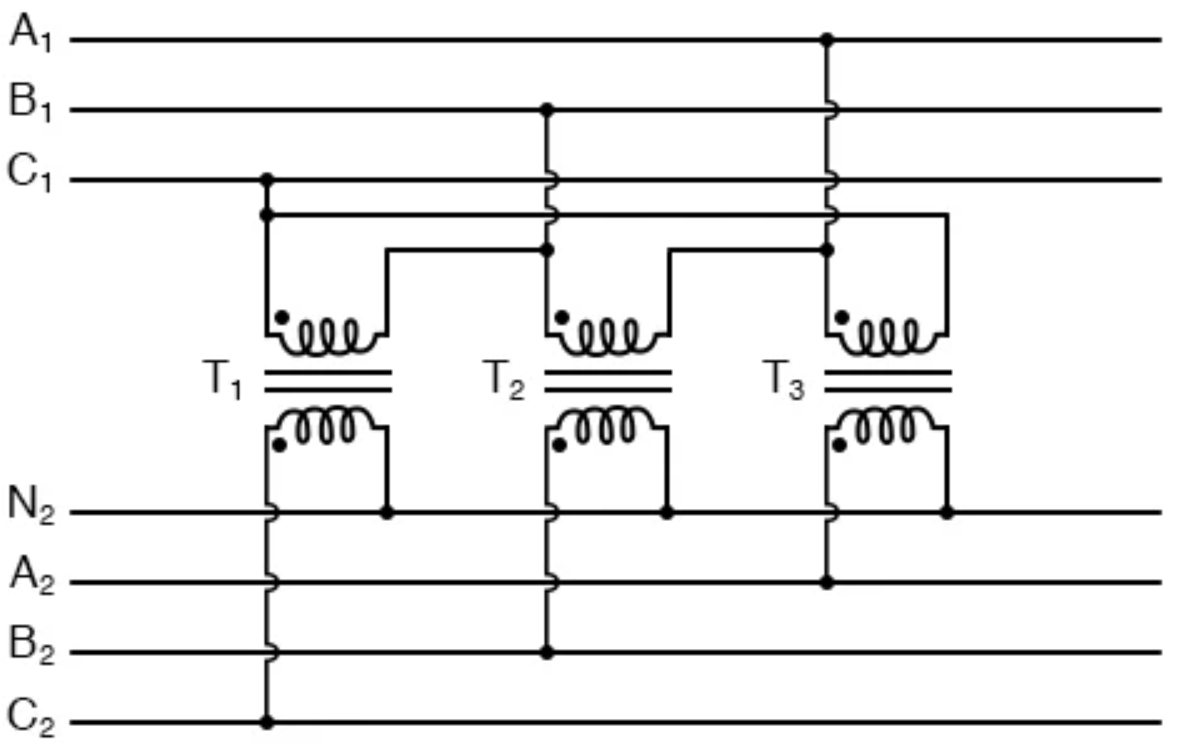
\includegraphics[width=0.6\textwidth]{delta-y.PNG}
    \caption{Delta-Star three-phase transformer}
    \label{fig:delta-star transformer}
    \end{figure}
    
    \item Star-Delta: The primary side is wired in star while the secondary side follows the delta configuration. Star-Delta transformers are often used for step-down transformer because high current will flows in the secondary side. Figure \ref{fig:star-delta transformer} depicts such configuration.  
    \begin{figure}[h]
    \centering
    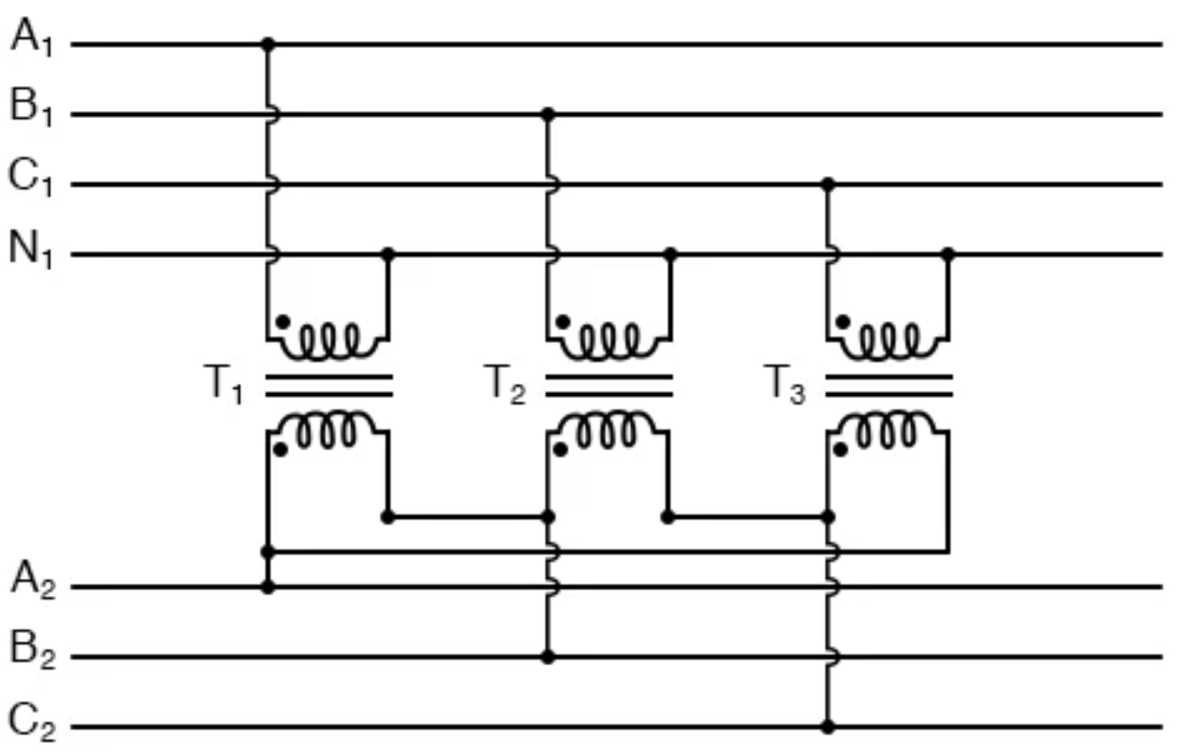
\includegraphics[width=0.6\textwidth]{y-delta.PNG}
    \caption{Star-Delta three-phase transformer}
    \label{fig:star-delta transformer}
    \end{figure}
\end{itemize}

Considering that the two studied transformers for this project are step-down transformers, the retain wiring configuration is the Star-Delta configuration.

\section{Nominal values}
\quad\, In the beginning of the chapter, the characteristics of the two transformers have been established. The nominal apparent power $S_N$ have been defined as being

\begin{equation}
\setstretch{1}
    S_N = \sqrt{3}\cdot U_{N,1}\cdot I_{N,1} = \sqrt{3}\cdot U_{N,2}\cdot I_{N,2}
\end{equation}

Therefore, considering the two transformers \textbf{A} and \textbf{B}, the nominal current that has to be sustained by the conductors can easily be obtained by replacing the nominal voltage and apparent power value by the ones in Table \ref{tab:characteristics_transfo}. The results of the calculations are included in Table \ref{tab:currents}.

\begin{table}[h]
    \centering
    \begin{tabular}{l|ll}
    Transformer                                  & \textbf{A} & \textbf{B} \\ \hline
    Nominal RMS current [A] - Primary side   & 48.11                       & 192.45                      \\
    Nominal RMS current [A] - Secondary side & 481.12                      & 4811.25                    
    \end{tabular}
    \caption{Primary and secondary currents of the two design}
    \label{tab:currents}
\end{table}


\section{Diameter of the windings}
\quad\, As it has been mentioned in the previous section, the conductors has to be designed such that the specified nominal currents can be sustained an infinite amount of time without causing damages.

It has been established that the maximum current density $J_{copper,max}$ of the copper is equal to 2 A/mm$^2$. Thus, by applying the formulae \ref{eq:Imax}, the cross-section of the conductors can be computed.

 \begin{equation}
 \setstretch{1}
    I_{1,2} =  J \cdot A_{1,2}\label{eq:Imax}
\end{equation}

Where $I_{1}=I_{N,1}$ and $I_{2}=\frac{I_{N,2}}{\sqrt{3}}$ since the current in each winding is $\sqrt{3}$ smaller than the current flowing through the lines.

Once the cross-section computed, the radius of the winding can be deduced. The Table \ref{tab:windings_A} includes the obtained results.
\begin{table}[h]
\centering
\begin{tabular}{l|llll}
Transformer             & \multicolumn{2}{c}{\textbf{A}} & \multicolumn{2}{c}{\textbf{B}} \\ \hline
Side                    & Primary       & Secondary       & Primary       & Secondary      \\
Nominal RMS current [A] & 48.11         & 481.12          & 192.45        & 4811.25        \\
Area [mm$^2$]           & 24.055        & 138.88          & 96.225        & 1388.88        \\
Radius [mm]             & 2.77          & 6.64            & 5.53          & 21.02         
\end{tabular}
\caption{Cross-section area of the windings}
\label{tab:windings_A}
\end{table}

As it can be noticed, the winding of the primary side are thinner than the one of the secondary side. This is logical because the current that has to be sustained is much higher in the low voltage side of the transformer.

\section{Number of winding turns}
\quad\, It has previously be defined the transformer ratio as being the ratio between the terminal secondary and primary phase-to-phase voltages of the transformer. Now, let's define the internal transformer ratio as being the ratio between the inner secondary and primary voltages of the transformer. The inner voltage is the one that would be measured at the winding terminals. 

By setting $n_1$ and $n_2$ as the number of turns of the primary and secondary winding, the internal transformer ratio $N_{int}$ is given by
\begin{equation}
    N_{int} = \frac{n_2}{n_1}=\frac{V_{2,int}}{V_{1,int}}
\end{equation}

Based on the previous statement, we can see that depending on the configuration of the transformer, the relation between the transformer ratio and the internal transformer ratio will be different. Considering the transformer as ideal, the relations for each configurations are listed in equations from (\ref{eq:N_star-star}) to (\ref{eq:N_delta-delta}).
\begin{subequations}
\setstretch{1}
\begin{equation}
    \bullet\text{Star-Star: } N_{int} = \frac{n_2}{n_1} = \frac{V_{2,int}}{V_{1,int}} = \frac{U_{2}}{U_{1}} = N\label{eq:N_star-star}
\end{equation}
\begin{equation}
    \bullet\text{Star-Delta: } N_{int} = \frac{n_2}{n_1} = \frac{V_{2,int}}{V_{1,int}} = \frac{U_{2}}{\frac{U_{1}}{\sqrt{3}}} = \sqrt{3}\cdot N\label{eq:N_star-delta}
\end{equation}
\begin{equation}
    \bullet\text{Delta-Star: } N_{int} = \frac{n_2}{n_1} = \frac{V_{2,int}}{V_{1,int}} = \frac{\frac{U_{2}}{\sqrt{3}}}{U_{1}} = \frac{N}{\sqrt{3}}\label{eq:N_delta-star}
\end{equation}
\begin{equation}
    \bullet\text{Delta-Delta: } N_{int} = \frac{n_2}{n_1} = \frac{V_{2,int}}{V_{1,int}} = \frac{U_{2}}{U_{1}} = N\label{eq:N_delta-delta}
\end{equation}\label{eq:N}
    \end{subequations}

Theses equations gives a relation between the ratio of the number of turns and the phase-to-phase terminal voltages of the transformer. Thus, if the number of the turns on one side is chosen, the number of turns at the other side will be deduced.

From the statement, it is asked to not exceed the saturation induction of the core. According to the Faraday's Law applied to one side of the transformer, the magnetic flux density $b$ is given by
\begin{equation}
\setstretch{1}
    b = \frac{V_{int}}{n\cdot\omega\cdot S} < 2
\end{equation}
where $\omega = 2\cdot\pi\cdot 50$ rad/s is the pulsation and S is the cross section of the core (in m$^2$). Usually, the number of turn is chosen at the side wired in star. Here, the primary side is in star configuration. So, the number of turns $n_1$ has to satisfy the inequality (\ref{eq:n_min}).
\begin{equation}
\setstretch{1}
    n_1 > \frac{V_{int}}{2\cdot\omega\cdot S}\label{eq:n_min}
\end{equation}

Also, assuming that there is no spacing between each turn in the winding, the number of turn is limited by the height of the core.

\section{Selection for core design}
\subsection{Comparison of core- and shell-type designs}
The most difference that exists between core- and shell-type design is that in core-type design the winding encircles the core as they are placed on two core limb and for shell-type design the core encircles most of the part of the windings as they are placed on mid arm of the core. That leads to single magnetic circuit in core-type while there are two magnetic flux paths for shell-type, as can be seen from Fig. \ref{fig:shell_core_type}.

 \begin{figure}[h]
    \centering
    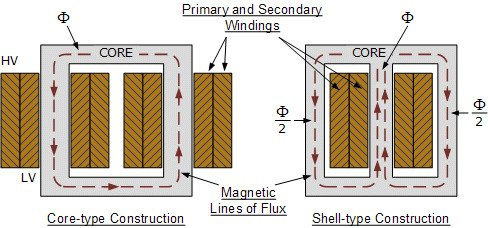
\includegraphics[width=0.6\textwidth]{type_design_2.jpg}
    \caption{Types of three-phase transformers design}
    \label{fig:shell_core_type}
\end{figure}


\subsection{Geometry of the design}
These designs have been performed using \textit{gmsh} and are shown in the Fig.\\
\textcolor{red}{+ ajouter les deux geos}

\begin{table}[h]
    \centering
\begin{tabular}{|l|l|l|l|l|}
  \hline
   & \multicolumn{2}{c|}{\textbf{Type A}} & \multicolumn{2}{c|}{\textbf{Type B}}\\\hline
   \textbf{Type design} & \textbf{Shell} & \textbf{Core} & \textbf{Shell} & \textbf{Core}\\\hline
   $N_1$ [turns]& & & &\\\hline
    $N_2$ [turns]& & & &\\\hline
    Width of the core [cm]& & & &\\\hline
    Thickness of the core [cm]& & & &\\\hline
    Total height of the transformer [cm]& & & &\\\hline
    Total width of the transformer [cm]& & & &\\
  \hline
\end{tabular}
    \caption{Geometry of the two three-phase transformers}
    \label{tab:designed_transfo}
\end{table}

+ Calculer les rendements des deux transfos :

\begin{equation}
   \eta = \frac{P_2}{P_1}
\end{equation}

\section{Transformer tests}

\subsection{Equivalent circuit}
There are two kind of tests : open and short circuit tests. They are both performed to determine the equivalent circuit of transformer, its voltage regulation and efficiency.
The power required for these tests is equal to the power loss occurring in the transformer.

 \begin{figure}[h]
    \centering
    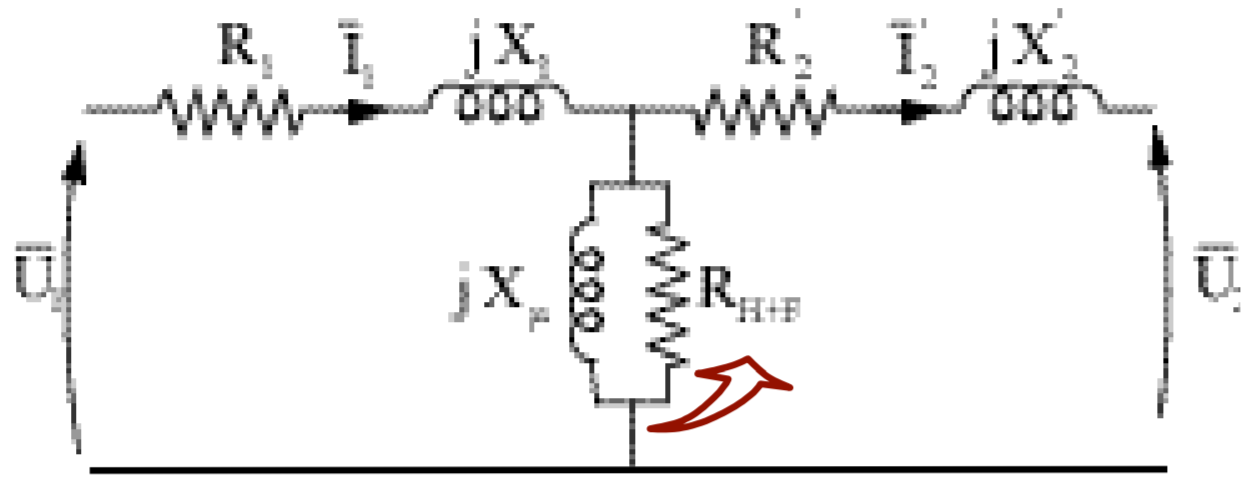
\includegraphics[width=0.6\textwidth]{equivalent_circuit.PNG}
    \caption{Transformer equivalent circuit}
    \label{fig:equivalent_circuit}
\end{figure}

\subsubsection{Open-load test}
Calculate the core loss Calcul des pertes dans le circuit magnétique  $R_{H,F}$ et $X_\mu$ :

\begin{equation}
   P_V = \frac{U_1^2}{R_{H,F}}
\end{equation}
\begin{equation}
   Q_v = \frac{U_1^2}{X_{\mu}}
\end{equation}

\subsubsection{Short-circuit test}
Calculate the total copper loss in the windings ,Calcul des résistances électriques des deux côtés + réactance de fuite :
\begin{equation}
P_{cc} = (R_1 + R_2') \cdot I_{cc}^2
\end{equation}
\begin{equation}
Q_{cc} = (X_1 + X_2') \cdot I_{cc}^2
\end{equation}

+ Tableau récapitulatif des valeurs

\subsubsection{Exterior characteristic}
Tracer le graphe caractéristique U-I pour chaque transfo

\section{Additional parametric studies}

\subsection{Effect of the winding electric resistivity}
Tracer le graphe de $\eta$ en fonction de $\rho$
\subsection{Effect of the core magnetic permeability}
Par exemple, tracer le graphe de $\eta$ en fonction de $\mu$
\subsection{Effect of the presence of an air gap}
Un air gap apporte une réluctance en série tel que :

\begin{equation}
    R_{fer} << R_{air}
\end{equation}
Vu que 
\begin{equation}
   R = \frac{1}{\mu} \cdot \frac{d}{S}
\end{equation}
et
\begin{equation}
   \mu_{fer} >> \mu_{air}
\end{equation}
Tracer le graphe de $\eta$ en fonction de l'air gap (< 0,1 mm)

\subsection{Effect of a non-laminated core}
Etant donné que le but du fer lamellé c'est diminuer les pertes par effet joule dûs aux courants de Foucault, on peut essayer de simuler du fer lamellé en faisant diminuer progressivement la conductivité électrique du noyau et voir l'impact sur le rendement $\eta$
--> graphe de $\eta$ en fonction de la conductivité $\sigma$
\subsection{Effect of shielding the transformer}
Shielding the transformer consists in surrounding it with a tank. +blabla\\

En pratique, rajouter une volume qui englobe le transfo dans la géométrie. Normalement, un bouclier n'augmente pas des masses le rendement du transfo.

\subsection{Effect of higher operating frequencies}
Calcul de la gamme de fréquence dans laquelle le transfo est censé fonctionner [$f_{min}$,$f_{max}$] + Que se passe-t-il si on augmente les 50 Hz ?\\

Par exemple, tracer le graphe de $\eta$ en fonction de $f$ ou $\omega$

\subsection{Effect of the loss of one phase}
%The effect of the loss of one phase also depends on the reasons for choosing a star or delta configuration for transformer winding connections. For example, star connections allows high range of voltages while delta connections are more reliable, meaning that if one winding stop working the other two can still maintain full line voltages to the load.

\section{Conclusion - Limitations - Further work}
Mettre les limites du modèle (cooling methods, insulating oil not discussed here, sélection du type d'enroulement selon la puissance apparente, ..)

\end{document}
